\documentclass[11pt]{article}

\usepackage{setspace}
\usepackage[margin=1in]{geometry}

% Make table of contents look better
\usepackage{tabularx}
\usepackage{tocloft}
\renewcommand{\cftsecleader}{\cftdotfill{\cftdotsep}}

\usepackage{graphicx}
\usepackage{pdfpages}
\usepackage{hyperref}

% \usepackage[ngerman]{babel}
% \usepackage[T1]{fontenc}
% \usepackage[ansinew]{inputenc}
% \usepackage{lmodern}

% Times New Roman font
\usepackage{txfonts}

\begin{document}

\setlength{\parindent}{2em}

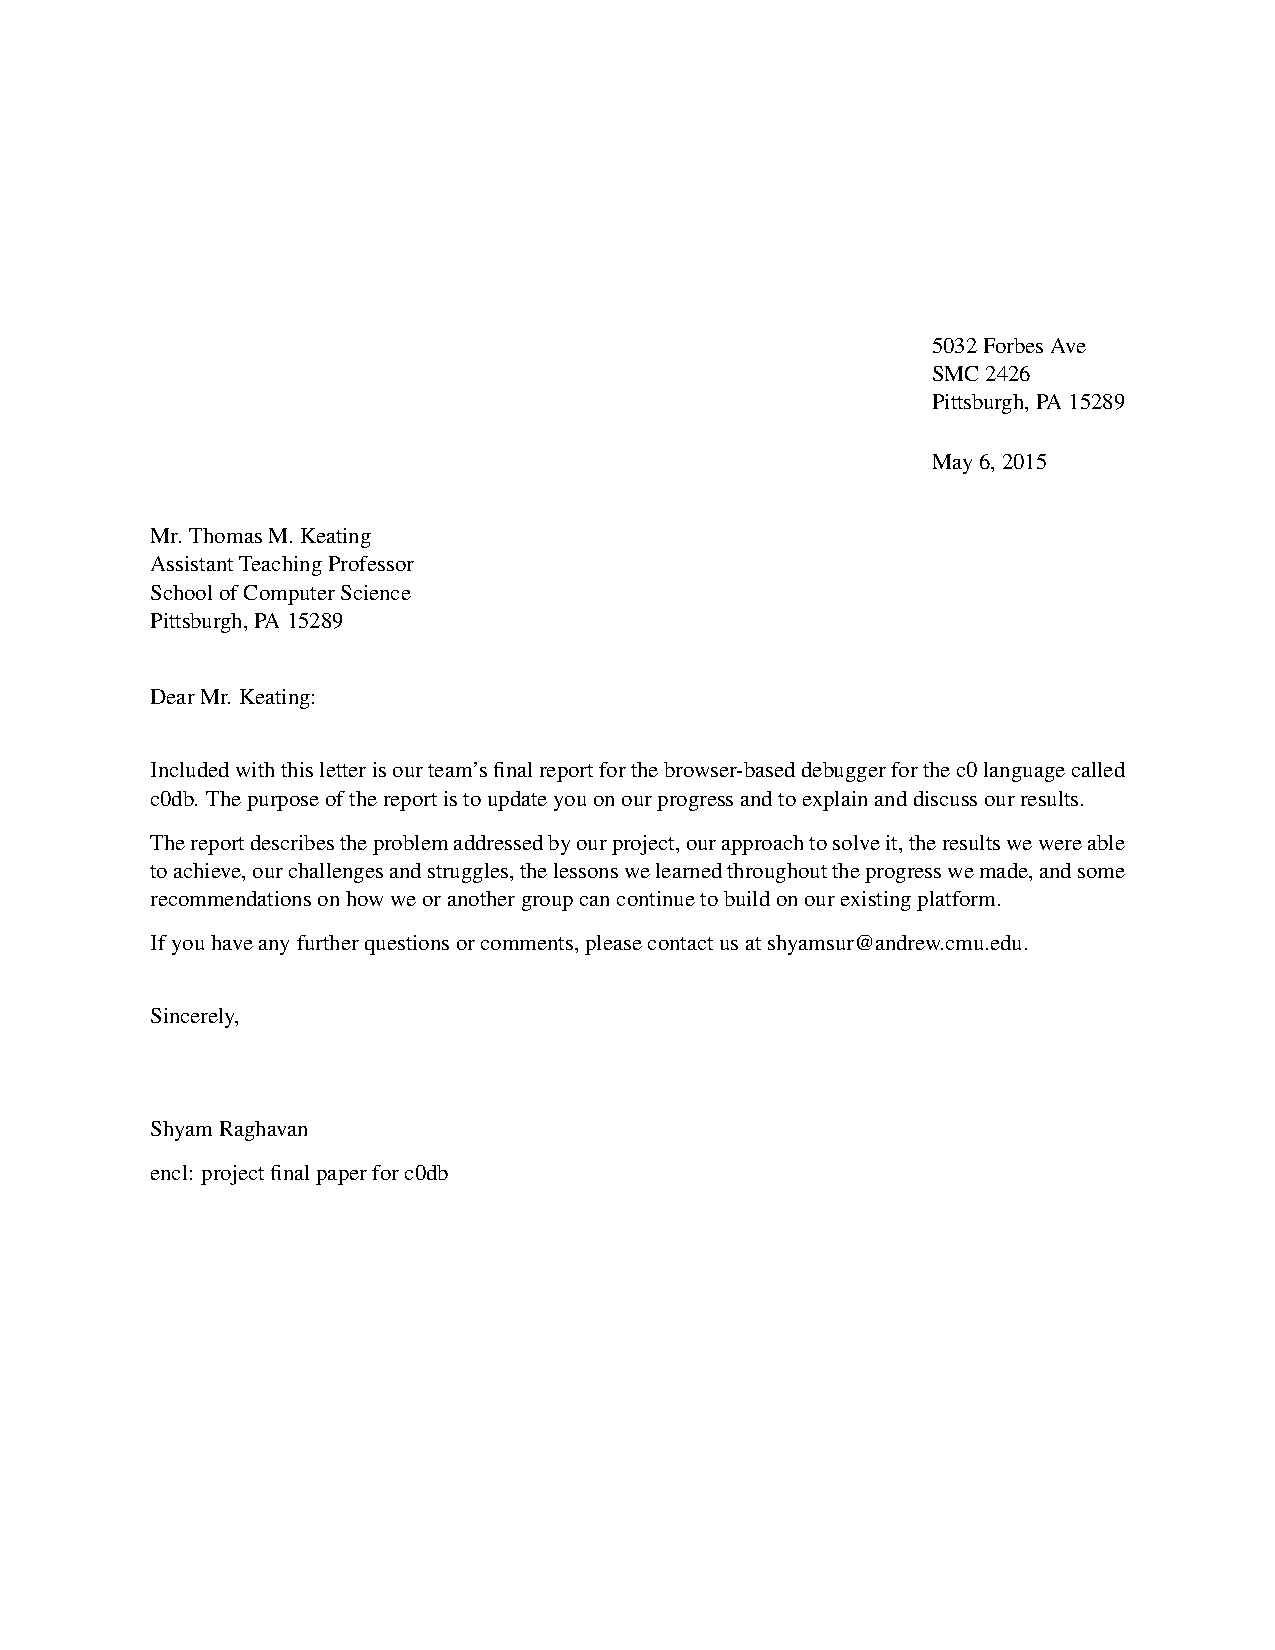
\includepdf[pages={1}]{letter.pdf}

\begin{titlepage}
\clearpage
\thispagestyle{empty}

\begin{center}
{\Huge Final Report}\\
\vspace{10 mm}
{\Huge {\tt c0db}\\[.4em]
The {\tt C0} Debugger}\\
\vspace{10 mm}

Submitted to\\
Mr. Thomas M. Keating\\
Assistant Teaching Professor\\
School of Computer Science\\
Carnegie Mellon University\\
Pittsbugh, PA 15289

\vspace{10 mm}

Prepared by:\\
{\bf Aaron Gutierrez}\\
{\bf Shyam Raghavan}\\
Mitchell Plamann\\
Suhaas Reddy

\vspace{10 mm}

School of Computer Science\\
Carnegie Mellon University\\
\today

\vspace{10 mm}

{\bf Abstract}
\end{center}
\par
Finding problems in code is a difficult and time consuming task, one especially
difficult for programmers learning a new language. To help students more quickly
find bugs and understand how their programs run, we created an online debugger
for the {\tt C0} programming language. The {\tt C0} debugger, {\tt c0db},
enables users to run programs in their browser and break apart the execution
when they don't run correctly.
\end{titlepage}

\pagenumbering{roman}
\tableofcontents
\newpage

\pagenumbering{arabic}

\section{Introduction}

\section{Approach}

\section{Results}
\par
We originally aimed to evaluate our performance against user feedback from both
current and past students. However, due to setbacks in the early stages of
development we were unable to receive significant use feedback from students.
That said, we were able to gather feedback and support from current 15-122
course staff.

In terms of our original vision, {\tt c0db} includes almost every feature we
planned to implement. Users can input code and either run the program straight
through or step through execution instruction by instruction. The only
significant feature that is not currently implemented completely is
breakpoints.  Implementing breakpoints turned out to be significantly more
difficult than we anticipated, and given our limited time frame, we were unable
to come up with an adequate solution. We are currently working with Rob
Simmons, 15-122 instructor and maintainer for the {\tt C0} language standard,
to extend the language to support breakpoints more easily going forward.

\begin{figure}[h]
  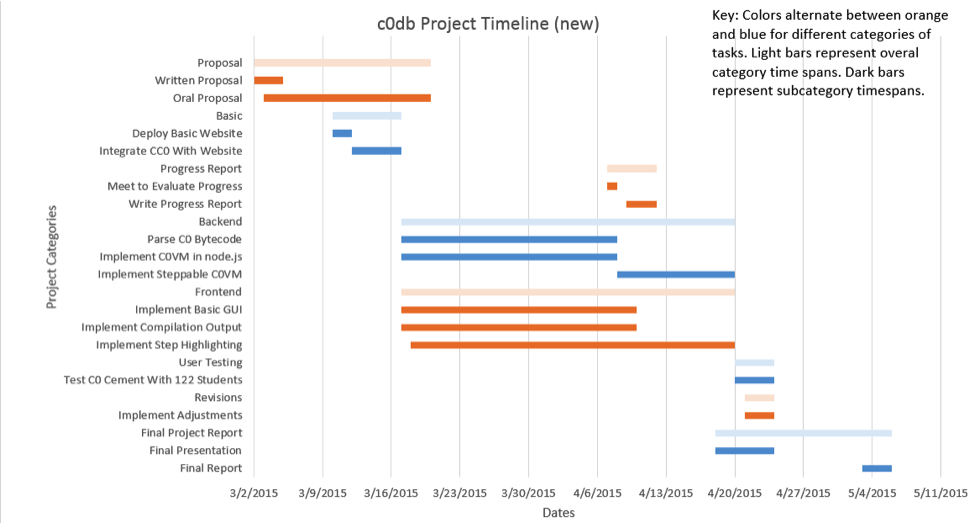
\includegraphics[width=\linewidth]{new-gantt}
  \caption{Revised project Gantt chart}
  \label{gantt}
\end{figure}
Relative to our revised Gantt Chart (Figure \ref{gantt}) we hit every milestone
on time. Both the front-end and back-end teams completed their tasks by the end
of April, at which point we transitioned everyone to user testing, revisions,
and polishing. Both teams were able to recover from the lag reported in our
progress report to complete {\tt c0db}.

\section{Discussion}

\section{Sources Cited}

\end{document}
